\section{Status}
\label{sec:implementation:status}

As part of the project we have designed and implemented a context-aware home automation solution on an Android Wear and a Raspberry Pi with Philips Hue light bulbs and a desktop machine running a Spotify client acting as the controllable devices. 

\Cref{fig:implementation:deployment-diagram} shows a deployment diagram of the prototype developed during the project. \Cref{sec:implementation:status:devices} describes the devices involved in the deployment as well as the features implemented on the devices.

In our specific prototype, we have a computer acting as the media centra and we have two Philips Hue light bulbs connected to openHAB. The number of devices will vary depending on the specific deployment, e.g. there can be more Philips Hue light bulbs or other devices in the system, e.g. door locks, a television or a thermostat.

\begin{figure}[H]
\centering
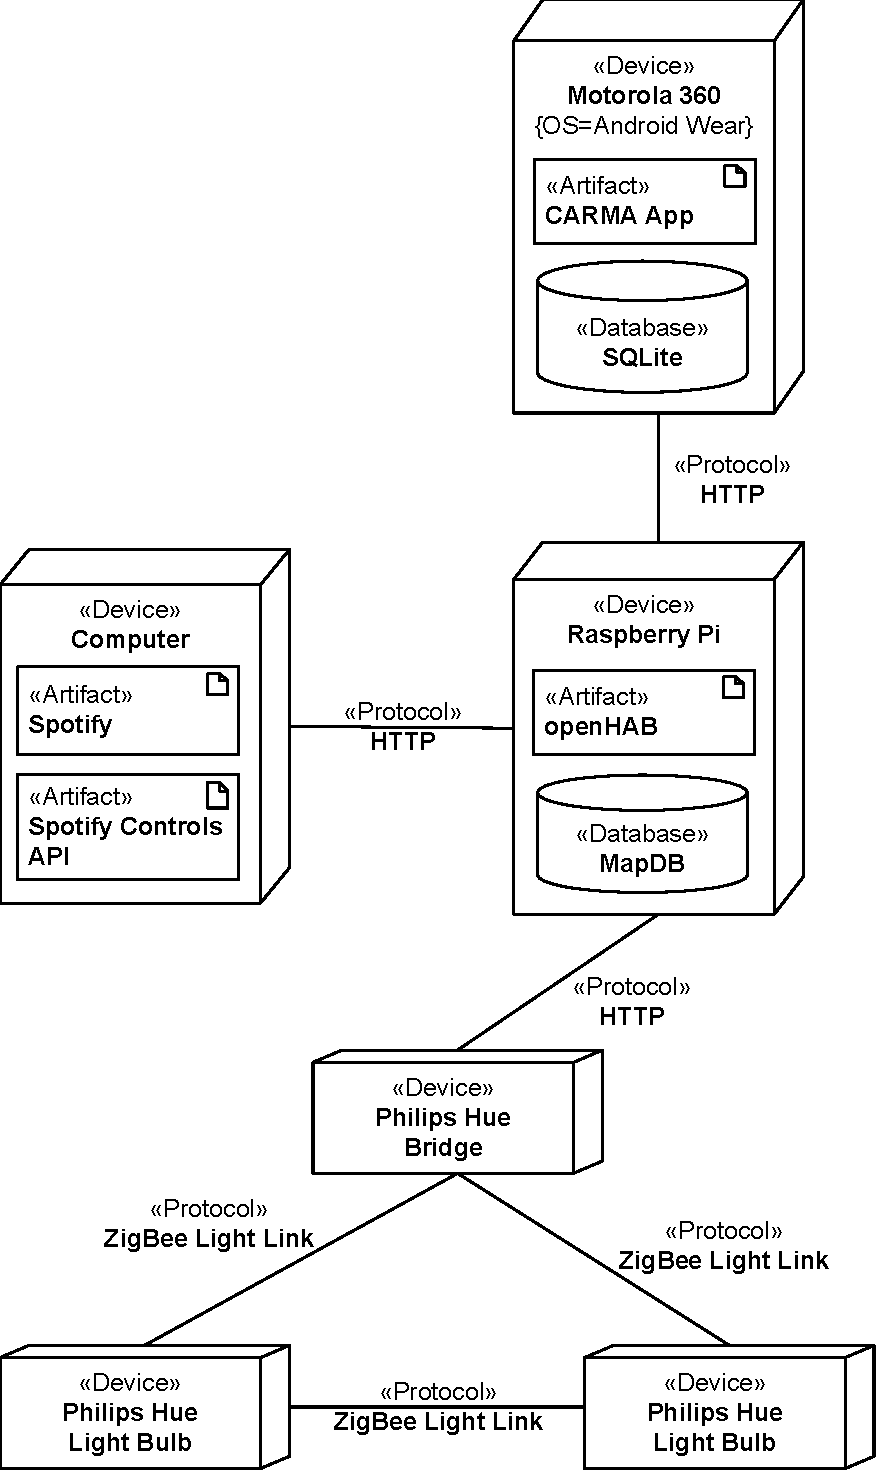
\includegraphics[height=0.95\textheight]{images/deployment-diagram}
\caption{Deployment diagram of the prototype developed in the project.}
\label{fig:implementation:deployment-diagram}
\end{figure}

\subsection{Devices}
\label{sec:implementation:status:devices}

Below we present the features implemented as part of the project. Features are grouped by the hardware the software is running on.

\subsubsection{Smartwatch}

The user utilizes the Android Wear smartwatch to perform gestures which starts the context recognition process. Furthermore the smartwatch is used for positioning the user and configuring parts of the system. The following features are implemented on the watch.

\begin{itemize}
\item Retrieval of available devices and actions from openHAB.
\item Configuration of the smartwatch application based on rooms and beacons registered in openHAB.
\item Training of gestures using the 1\textcent~gesture recognizer as described in \Cref{sec:design:gesture-recognition}.
\item Recognition of gestures using the 1\textcent~gesture recognizer.
\item Positioning of the user using Estimotes BLE beacons as described in \Cref{sec:design:ble-positioning}.
\item Setup of gesture configurations, i.e. a combination of a gesture, a room and an action.
\item Recognition of the context using a Bayesian network as described in \Cref{sec:design:bayesian-network}.
\item Presentation of a list of actions if one single action cannot be determined but rather we have a set of actions to choose from.
\item Configuration and use of virtual positions, i.e. allowing the user to manually determine which room he is in.
\end{itemize}

\subsubsection{BLE Beacon}

The Bluetooth Low Energy beacons are used to position the user indoor.

We have not implemented any features on the BLE beacons but in order to position te user, the smartwatch reads the RSSI values from the Bluetooth beacons and based on those values determines which room the user is in, described in detail in \Cref{sec:design:bayesian-network:room-node-evidence}.

\subsubsection{Raspberry Pi}

The Raspberry Pi runs openHAB, which was described in \Cref{sec:analysis:choice-of-hub}. openHAB is the home automation software utilized in the project. The software receives HTTP requests usoing an HTTP API. The request is then translated to an equivalent request using an appropriate protocol, e.g. Bluetooth, HTTP or MQTT, and forwards the translated request to a controllable device. The following features were implemented on openHAB.

\begin{itemize}
\item We implemented an openHAB plugin for configuring which beacons are installed in the rooms of the users house or apartment.
\item openHAB was configured to support the actions in the scenario presented in \Cref{sec:analysis:scenarios}, e.g. we implemented rules to toggle a lamp between the on and off states as this is not directly supported by openHAB.
\end{itemize}

\subsubsection{Computer}

The desktop machine serve as the media centre used for testing while developing the solution. In order to control Spotify, we developed a smart application that runs on the desktop machine. The application receives requests over HTTP and forwards them to the Spotify client for OS X which is an AppleScript scriptable application, meaning that it provides a terminology that scripts can use to send \emph{events} to the application. An event triggers a handler within the application which in some way modifies the application. For the Spotify application, events includes ``next'', ``previous'' and ``playpause''. When the application receives an event, an appropriate action is taken in the application.

The following feature was implemented in the application running on the desktop machine.

\begin{itemize}
\item Skip to next track, skip to previous track, play and pause the music in Spotify by issuing HTTP requests to the application.
\end{itemize}

\subsubsection{Philips Hue Bridge}

A bridge provided by Philips is installed in the users home. The bridge communicates with the Philips Hue lights using the ZigBee protocol. The protocol is described later in this section.

We have not implemented any features on the bridge but use it in order to control the Philips Hue light bulbs.

\subsubsection{Philips Hue Light Bulb}

The light bulbs provided by Philips are controlled using gestures on the smartwatch, i.e. using the CARMA application. The bulbs receive commands from the Philips Hue bridge when they need to change their state, e.g. turn on, turn off, change color or change temperature. The bulbs can communicate with each other using the ZigBee Light Link protocol to extend the range of the network by forwarding commands between bulbs.

\subsection{Known Issues}

The following describes known issues in the implementation.

\begin{itemize}
\item There is an issue with the implementation of the gesture recognizer that causes the smartwatch application to crash if recognition is started with little to no measurements from the accelerometer are available to the gesture recognizer. In order to fix the issue, recognition should most likely be abandoned all together when little information is available. We have only seen the issue when users have accidentally stopped recognition immediately after starting it.
\item Sometimes the application will hang, i.e. ``freeze'', when context recognition is started. The fix for the issue is most likely to perform the context recognition on another thread.
\item In order to present the settings (see \Cref{fig:implementation:prototype:screenshots:3}), the user must scroll from right to left on the gesture recognition screen (see \Cref{fig:implementation:prototype:screenshots:1}). The list of settings is meant to be scrolled vertically but it seems that the horizontal scroll gesture interferes with the vertical scroll causing the list of settings not to scroll. It is, however, possible to tap in the top and the bottom of the list to change the selected setting.
\end{itemize}

\subsection{Missing Implementation}

While not part of the requirements presented in \Cref{sec:requirements-specification}, we presented a model for including the state of the system in \Cref{sec:design:bayesian-network}. The system state was introduced in the model to illustrate how contextual information different than the gesture performed by the user and the users location can be included in the system.

The following features were not implemented.

\begin{itemize}
\item Inclusion of the system state in the Bayesian network used for recognizing the context.
\item Reuse of the Bayesian network. The Bayesian network is created every time the recognition is started. When the network is created once, it could be reused for future computations of beliefs.
\end{itemize}

While inclusion of the system state is not implemented, a naive implementation of the system state is trivial to implement. The Android Wear application can periodically request the state of all controllable devices registered in openHAB and based on the response, populate the system state nodes in the Bayesian network with the appropriate states. The nodes will typically have hard evidence on one of the states as openHAB is considered to hold the truth of the systems state, e.g. it knows if a television is on or not and if music is playing or not.

Reuse of the Bayesian network could be implemented by creating the network when the application whenever the network changes, i.e. new gesture configurations are created. The network could then be stored either in memory or on disk and loaded. For sufficiently large networks, this may be faster than recreating the network whenever it is needed.

\subsection{HTTP}

As shown in \Cref{fig:implementation:deployment-diagram} we use HTTP for communication between the smartwatch, the Raspberry Pi and the computer acting as media centre.

HTTP, or Hyptertext Transfer Protocol, which it is short for, is a protocol generally used for exchanging \emph{hypertext}, text which includes hyperlinks. HTTP is a client-server protocol, in which a client sends a request to the server which in turn sends a response.

Resources provided by the server are identified by a URL, a Uniform Resource Locator. An example of a URL is ``http://mysite.com/index.html'' which requests the ``index.html'' file on the ``mysite.com'' hostname using the ``http'' protocol.

When a web server returns a response, it will return an HTTP status code as part of the response. Examples of this includes the status code 200 for success, 404 for a resource not found and 400 for a bad request.

HTTP utilize TCP/IP to transfer information. TCP transfers information in small packets between machines and IP is responsible for addressing machines in a network and routing the information between the machines.

In our prototype we use a framework appropriate for the platform to issue requests and send a response, e.g. in the case of the smartwatch application we use the Android Volley framework for making requests\footnote{For more information about Google Volley, refer to \url{https://developer.android.com/training/volley/}}. In the case of the Spotify Controls API, we use the Express\footnote{For more information about Express, refer to \url{http://expressjs.com}} framework for building the server.

The requests are sent to either openHAB or the Spotify Controls API which will return a response formatted using JSON. In the case of a simple request, e.g. for changing the state of the music centre, the JSON response, as well as the HTTP status code, indicates whether or not the request was successful. For a more complex request, e.g. when requesting the available items in openHAB, the response will contain all available items in openHAB formatted as JSON along with a HTTP status code.

HTTP defines methods for sending requests to a server. Amongst others are GET, POST and PUT, which are generally used for retrieving content,creating content and updating existing content, respectively. The Spotify Controls API use the HTTP method PUT for changing the state of the player. 

Likewise the openHAB API also use the GET, POST and PUT where appropriate.

% \subsection{ZigBee}

% The ZigBee protocol is targeted towards devices that fit within the concept of internet of things, e.g. lamps, thermostats and door locks. The devices create a \emph{mesh network}, i.e. a network in which nodes relays information to other nodes \cite{zigbee:zigbee-pro}. This is depicted in the deployment diagram shown in \Cref{fig:implementation:deployment-diagram} in which both Philips Hue light bulbs receives commands by the bridge but the bulbs can also relay commands to each other.

% The ZigBee protocol, amongst others, specifies the frequencies on which the devices shuld communicate, how devices are discovered and how they are paired with each other.

% The Philips Hue light bulbs used in our prototype utilize the ZigBee Light Link standard, an extension of the ZigBee protocol, which is a ZigBee standardization of how communication with light bulbs is done, e.g. the information sent to the bulbs when changing their state.

% In this project, we have not implemented communication using ZigBee, but instead utilize HTTP to communiate with the Philips Hue brdige which in turn communicates with the bulbs using the ZigBee protocol.

%%% Local Variables:
%%% mode: latex
%%% TeX-master: "../../master"
%%% End:
